% Chapter Template

\chapter{System Implementation} % Main chapter title

\label{Chapter5} % Change X to a consecutive number; for referencing this chapter elsewhere, use \ref{ChapterX}

\lhead{Chapter 5. \emph{System Implementation}} % Change X to a consecutive number; this is for the header on each page - perhaps a shortened title
In this chapter the implementation of various components specific to the experimental platform taking advantage of the framework proposed in \ref{Chapter4} is presented. The software is designed using a layered hierarchical structure. The various layers of the system are
\begin{itemize}
\item \emph{Hardware Layer} is composed of sensors and robots connected to the network. Currently only those sensors that support TCP/IP network communication are considered.
\item \emph{Distributed Components Layer} is composed of individual processes that could be running across different computers/devices in the network
\item \emph{Application Components Layer} is the central server of the experimental platform
\item \emph{User Interface Layer} takes the responsibility of providing useful and intuitive user-interface to the end users.
\end{itemize}
The architecture of the system shown in Fig~\ref{fig:architecture}. More finer details of each of the layers are presented in the following Sections~\ref{ssec:app_comp}$\sim$\ref{ssec:ui_comp}.
\begin{figure}
\centering
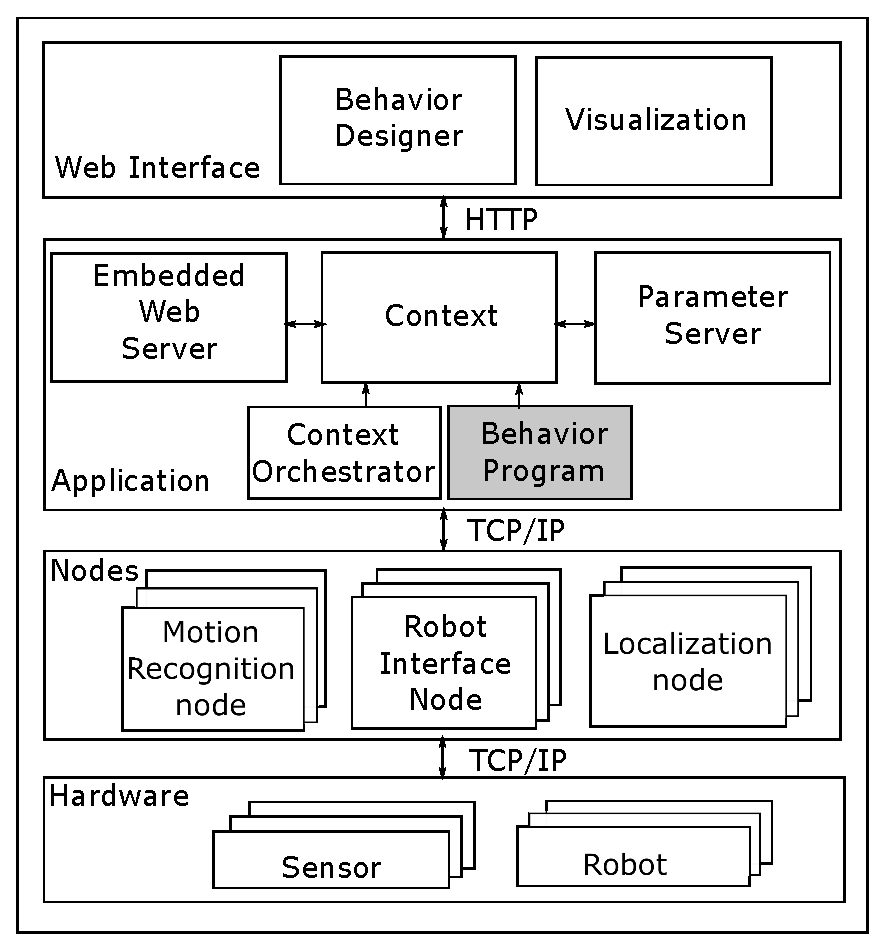
\includegraphics[width=\textwidth]{assets/architecture.eps}
\caption[System Architecture]{System Architecture}
\label{fig:architecture}
\end{figure}
\section{Application Components}
\label{ssec:app_comp}
The application level components are responsible for bootstrapping and maintain the uptodate status of the system. 
\subsection{Context}
The application context contains the complete description of the world. It contains latest information about
\begin{itemize}
\item Robot(s): A list of robots in the environment along with their 6D pose, Sensor information like Joint values etc.,
\item Human(s): A list of humans with their Skeleton Positions and Orientation, Active Gestures/Motions
\item Object(s): A list of manipulable objects in the environment along with their properties like description, color etc.,
\item Gesture Modules : A set of gesture recognition modules registered in the system that can actively provide information about the gestures of the humans in the environment.
\item Robot Behavior Modules: A set of robot behavior execution modules registered in the system.
\end{itemize}
The data structure of the context is shown in Fig~\ref{fig:system_context}
\begin{figure}
\centering
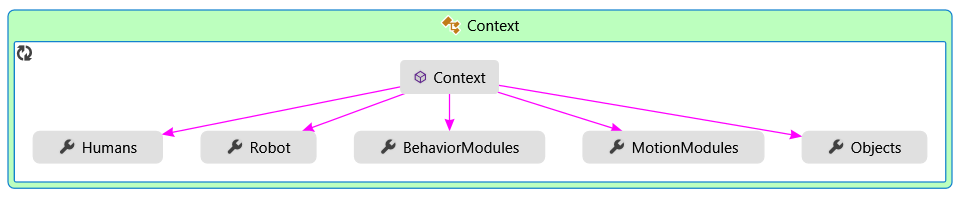
\includegraphics[width=\textwidth]{assets/context_diagram.png}
\caption[Application Context]{Application Context}
\label{fig:system_context}
\end{figure}
\subsection{Parameter Server} 
The parameter server acts as a central repository for managing the parameters of the system and of the distributed components. The parameter server is basically desgined as a responder socket which responds to the requests from a remote client. The list of supported request to pull the data from the parameter server is shown in the Table~\ref{table:parameter_server}
\begin{table}
\centering
\small
\caption{Parameter Server Interface Specification}
\label{table:parameter_server}
\begin{tabularx}{\linewidth}{c*3{X}}
\toprule
  \textbf{Request Description} & \textbf{Request Arguments}
                          & \textbf{Response}
  \tabularnewline \midrule
  \multirow{1}{*}{Node Parameters req} & Name of the node & Node Parameters 
                                          \tabularnewline\midrule
                                          
  \multirow{3}{*}{Motion recognition module registration req} & Name of the node; & Registration Status  \\
                                                     & Module Information &  (Success/Failure)
                                          \tabularnewline\midrule
  
  \multirow{3}{*}{Robot Interface module registration req} & Name of the node; & Registration Status  \\
                                                     & Module Information &   (Success/Failure)
                                          \tabularnewline\midrule
  \multirow{1}{*}{File Request} & Name of the file & Contents of the File  
  										 \tabularnewline                       
                                         
  										\bottomrule
\end{tabularx}
\end{table}
\subsection{Context Orchestrator} The orchestrator collect uptodate information about the robots and humans in the environment from the perception system and updates the Context. The algorithm used by the Orchestrator to update the context information is shown below.
\begin{algorithm}
 \KwData{(app\_config, context)}
 \textbf{\emph{Init}}:\\
 \quad PUBLISHERS = READ\_ALL\_PUBLISHER\_INFO(app\_config)\;
 \quad SUBSCRIBERS = CREATE\_SUBSCRIBERS(PUBLISHERS)\;
 \While{run}{
 	\ForAll{SUBSCRIBER in SUBSCRIBERS}{ 
 		data = RECEIVE\_DATA(SUBSCRIBER,TIME\_OUT)\;
 		UPDATE\_CONTEXT(context, data)\;
 	}
 }
 \caption{Context Synchronization Algorithm}
 \label{alg:context_sync}
\end{algorithm}
\subsection{Embedded Web server}
The web server embedded in the application serves the file and data requests from the web client. The server side server implements a set of RESTful services which could be accessed from the web clients. The JSON data format which the default standard for modern web interface development has been adopted. The list of RESTful API implemented on the server side is shown in Table~\ref{table:restful_api}
\begin{table}
\centering
\small
\caption{Embedded Web Server RESTful API}
\label{table:restful_api}
\begin{tabularx}{400pt}{c*4{X}}
\toprule
  \textbf{Request Url}  & \textbf{Parameters} & \textbf{Request Type} & \textbf{Description/Response}
  \tabularnewline \midrule
  \multirow{1}{*}{/models/{type}/(?$<$all$>$.*)} & File Name & GET & Robot 3D Model Data
                                          \tabularnewline\midrule
                                          
  \multirow{1}{*}{/context}  & - & GET & Current context data  
  										 \tabularnewline\midrule
  										 
  \multirow{1}{*}{/robot}  &  - & GET & Default Robot information  
  										 \tabularnewline\midrule										 
  
  \multirow{2}{*}{/humans} & - & GET  & Information about all the human in the environment  
                                          \tabularnewline\midrule
                                          
  \multirow{2}{*}{/human/{id}} & id - Human Id & GET  & Information about the human with the given id.  
                                          \tabularnewline\midrule
                                          
  \multirow{2}{*}{/jointvals} & - & GET  & Joint values of the default robot  
                                          \tabularnewline\midrule
                                          
  \multirow{3}{*}{/visualize/skeleton/list} & - & GET  & 3D Skeleton positions of all the humans in the environment  
                                          \tabularnewline\midrule                                        
       
  \multirow{3}{*}{/designer/program/list} & - & GET  & List of all the behavior programs stored in the server  
                                          \tabularnewline\midrule                                                               
  \multirow{3}{*}{/visualize/skeleton/list} & - & GET  & 3D Skeleton positions of all the humans in the environment  
                                          \tabularnewline\midrule                                       
                                          
  \multirow{3}{*}{/designer/program/startxml} & Behavior Program & POST  & Request the bootstrapper to start the program
  										 \tabularnewline\midrule   
  \multirow{3}{*}{/designer/program/save} & File Name & POST  & \\
                                          & Behavior Program &  & Request the bootstrapper to start the program
                                          \tabularnewline\midrule 
  \multirow{3}{*}{/designer/program/stop} & - & POST  & Request to stop running program if any
                                          \tabularnewline
                                                                                                                         
  										\bottomrule
\end{tabularx}
\end{table}
\subsection{Behavior Program} 
A dynamic component that will be created when the user starts the program he/she designed using the user interface. The declarative description of the behavior is parsed in order to create a memory model. The Behavior program node monitors the application context for the motion triggers and invokes the corresponding robot actions according to the way it is being described in the program.
\subsection{Bootstrapper} 
The bootstrapper takes care of initializing the system and starting up all the pre-configured nodes. It also takes of starting and stopping the behavior programs when requested by the user. The sequence operations of bootstrapper performs is represented in Algorithm~\ref{alg:bootstrapper}.
\begin{algorithm}
 \KwData{(app\_config)}
 \textbf{\emph{Startup}}:\\
 \quad INIT\_AND\_RUN\_PARAMETERSERVER()\;
 \quad INIT\_AND\_RUN\_CONTEXTSYNC()\;
 \quad INIT\_AND\_RUN\_CONTEXTSERVER()\;
 \quad INIT\_AND\_RUN\_WEBSERVER()\;
 \quad NODES = GET\_NODES(app\_config)\;
 \quad PROCESSES = []\;
 \ForAll{NODE in NODES}{ 
 	\If{NODE is ENABLED}{
 		PROCESS = CREATE\_PROCESS(NODE)\;
 		APPEND(PROCESSES, PROCESS)
 	} 
 }
 \While{run}{
 	MONITOR(PROCESSES)
 }
 \textbf{\emph{Shutdown}}:\\
 \quad SHUTDOWN\_WEBSERVER()\; 
 \quad SHUTDOWN\_CONTEXTSERVER()\;
 \quad SHUTDOWN\_CONTEXTSYNC()\;
 \quad SHUTDOWN\_PARAMETERSERVER()\;
 \quad SHUTDOWN(PROCESSES)
 \caption{Bootstrapper Algorithm}
 \label{alg:bootstrapper}
\end{algorithm}
\section{Distributed Components}
\label{ssec:dist_comp}
These are nodes in the system each with a specific goal that can be started/stopped at any time during the entire application life-cycle without affecting the other nodes or the system. All the nodes will communicate with the application using message passing techniques. They can run in any machine inside the network.

\subsection{Motion Recognition Node} A dedicated node that interacts with a motion recognition sensor and sends the detected gestures and motions to the application. Additionally each motion recognition module registers a set of actions/gestures that could be detected with the sensor associated with it. The gesture recognition logic depends on the sensor associated with the gesture recognition module. The gesture recognition workflow of kinect based system in explained in Section~\ref{sssec:kinect_gestures}
\subsubsection{Kinect Gesture Recognition}
\label{sssec:kinect_gestures}
	The Microsoft Kinect system utilizes Adaptive Boosting(adaboost) algorithm \cite{freund1997decision} is used to efficiently detect the gestures. The system involves a training phase in which the desired gestures are captured and tagged. These tagged gestures will be used by a gesture detector trainer which will generate a set of training examples. The training results are stored in files and will be used by the gesture detector to perform per-frame classification of the data. The Visual Gesture Builder (VGB) tool that comes together with Kinect for Windows SDK eases the process of tagging the gestures and creating the gesture database. The work-flow of using the VGB is shown in the Figure~\ref{fig:vgb_workflow}.
\begin{figure}
\centering
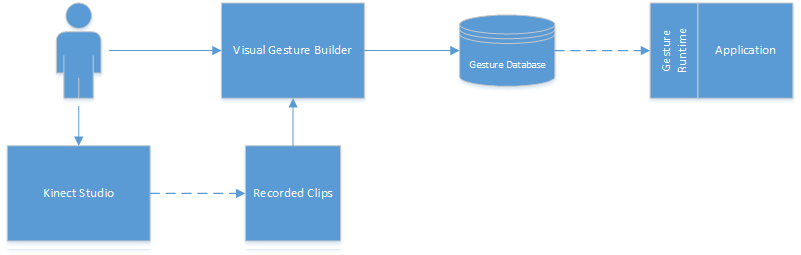
\includegraphics[width=\textwidth]{assets/VisualGestureBuilder.png}
\caption[Visual Gesture Builder Work flow]{Visual Gesture Builder Work flow \cite{KinectSDK2014}}
\label{fig:vgb_workflow}
\end{figure}
% Motion recognition
\begin{algorithm}
 \KwData{Gesture database}
 \KwResult{Gesture Triggers}
 \textbf{\emph{Init}}:\\
 \quad gestures = READ\_DATABASE()\;
 \quad REGISTER\_GESTURES(gestures)\;
 \While{True}{
 	skeletons = GET\_SKELETONS()\;
 	\ForAll{gesture in gestures}{ 
 		detected = DETECT\_GESTURE(gesture)\;
 		\If{detected}{
 			PUBLISH(gesture)\;
 		} 
 	}
 	PUBLISH(skeletons)\;
 }
 \caption{Kinect Gesture Recognition Module}
 \label{alg:localize}
\end{algorithm}
The workflow shown in Figure~\ref{fig:vgb_workflow} has been adopted to develop all the gestures needed for the kinect gesture recognition module. The process followed for generating the Left hand wave gesture is shown in the Figure~\ref{fig:gesture_waveleft}
\begin{figure}
\centering
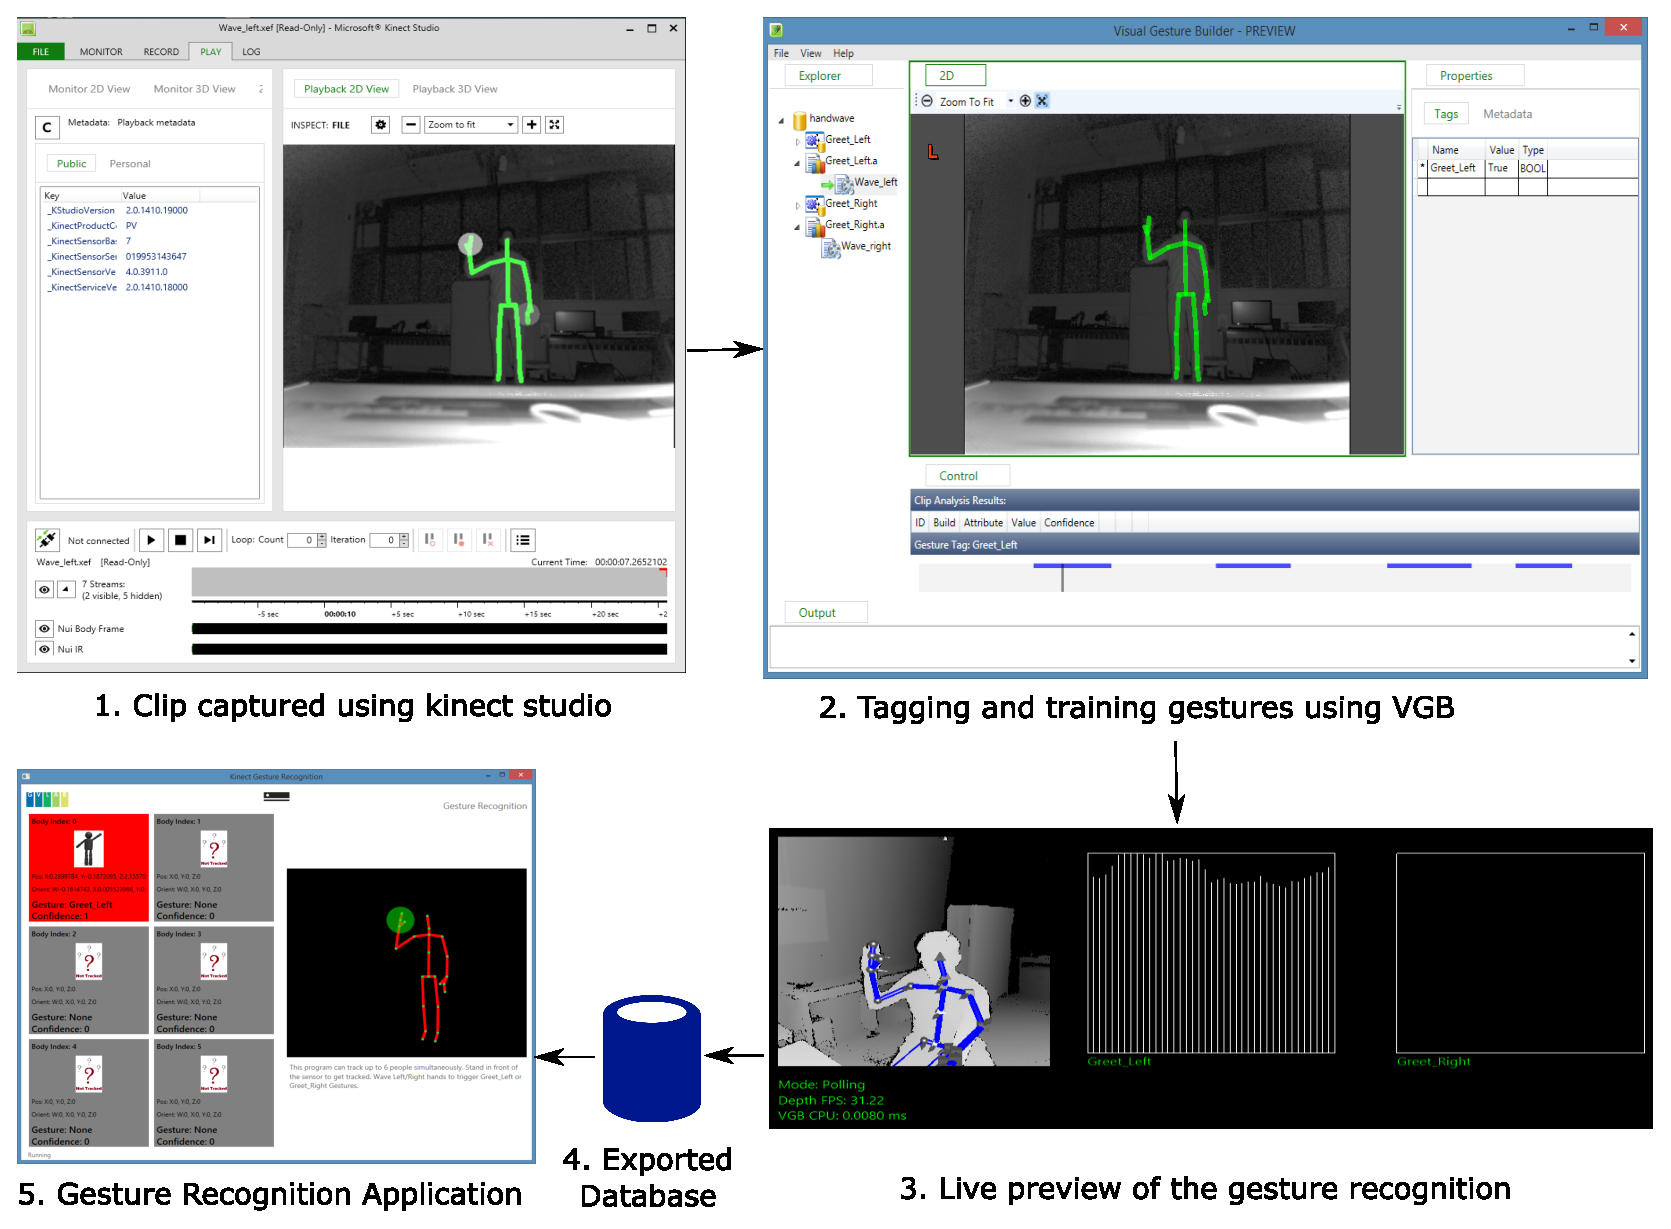
\includegraphics[width=\textwidth]{assets/gesture_recog_flow.eps}
\caption[Left hand wave gesture work flow]{Left hand wave gesture work flow}
\label{fig:gesture_waveleft}
\end{figure}
\subsection{Robot Interface Node} 
	The Robot Interface node is a dedicated node that interacts with a specific robot and can invoke a set of actions on it.  It registers a set of actions that could be invoked on the robot associated with it. The robot interface node sets up a publisher that periodically sends the information about the robot status like joint values, sensor information to the application to keep the context uptodate. Additionally it sets up a responder socket which will wait for action execution request from the remote node. The robot interface node dedicated to Nao humanoid robot is described in Section~\ref{sssec:nao_interface}
\subsubsection{NAO Robot Interface}
\label{sssec:nao_interface}
	
\subsection{Localization Node} A dedicated node which uses the perception system to resolve and publish the current position of the robot and the human which is very important for interaction.

\begin{algorithm}
 \KwData{Marker\_size, Cube\_size, MDH\_Params}
 \KwResult{TORSO\_POSE}
 \textbf{\emph{Init}}:\\
 k\_model := INIT\_MDH\_PARAM(MDH\_Params)\;
 m\_model := MARKER\_MODEL(Marker\_size, Cube\_size)\;
 \While{True}{
 	data = READ\_SENSOR()\;
 	marker\_poses = DETECT\_MARKERS(data)\;
 	$^{W}{T}_{M}$ = TRANSFORM\_TO\_TOP\_FRAME(marker\_poses, m\_model)\;
 	[$head_{yaw}$,$head_{pitch}$] = READ\_JOINT\_VALUES()\;
 	$^{T}{T}_{M}$ = COMPUTE\_TOP\_FRAME(k\_model,$head_{yaw}$,$head_{pitch}$)\;
 	$^{W}{T}_{T}$ = $^{W}{T}_{M} \times {^{T}{T}_{M}}^{-1}$\;
 	TORSO\_POSE = MEDIAN\_FILTER($^{W}{T}_{T}$)\;
 	PUBLISH(TORSO\_POSE)\;
 }
 %\caption{Localization Algorithm}
 %\label{alg:localize}
\end{algorithm}


\section{User Interface}
\label{ssec:ui_comp}
The user interface is a web application that runs on any latest web-kit browsers supporting WebGL technology. 

\subsection{Behavior Designer} The Behavior designer surface could be used by the user to drag and drop the behavior blocks and construct the program using the set of motion capabilities registered by the active motion recognition nodes and the set of robot action capabilities registered by the active robot interface nodes. The behavior designed using the designer will be encoded into a declarative XML format and sent to the server when the user request to start the program. The designer offers a full range of capabilities like Create/Edit/Delete/Save behavior programs.
\subsection{Visualization} The visualization could be used to see the interaction of the human and robot inside a virtual 3D environment.
% Simulation Node
\begin{algorithm}
 \KwData{simulation\_config}
 \textbf{\emph{Init}}:\\
 \quad INIT\_SIMULATION\_ENGINE(simulation\_config) \;
 \quad INIT\_SUBSCRIBERS(simulation\_config) \;
 \quad LOAD\_ENVIRONMENT(simulation\_config) \; 
 \While{True}{
 	sensors = READ\_SENSOR\_VALUES() \; 
 	skeletons = READ\_SKELETON\_DATA() \; 
 	RENDER(robot,sensors)
 }
 %\caption{Localization Algorithm}
 %\label{alg:localize}
\end{algorithm}


